\documentclass[UTF8]{article}
\usepackage{ctex}
\usepackage{amsmath}
\usepackage{graphicx}
\usepackage{listings}
\usepackage{color}
\usepackage{geometry}
\usepackage{caption}
\usepackage[dvipsnames]{xcolor} % 更全的色系
\usepackage{listings} % 排代码用的宏包
\usepackage{svg}
\usepackage{subcaption}
\usepackage{hyperref}
\usepackage[linesnumbered,ruled,vlined]{algorithm2e}
\geometry{a4paper, margin=1in}

% Title and Author
\title{​Chapter 6 Color Image Processing}
\author{李想 \quad P12214061}

\begin{document}

\maketitle
\section{问题一}
彩色图像进行直方图均衡化,首先想到将彩色图像的各个通道
分别均衡化,但这种方法会产生错误的彩色。更合适的做法是
,均匀地分布颜色亮度,而保持颜色本身(色调)不变。HSI
彩色空间是适合直方图均衡化的理想空间。
\subsection{RGB to HSI}
已知一幅RGB彩色格式的图像,每个RGB像素的 I 分量可由
公式(\ref{eq:1})得到:
\begin{equation}
    I = \frac{1}{3}(R + G + B)
    \label{eq:1}
\end{equation}
饱和度分量 H 为:
\begin{equation}
    S = 1 -\frac{3}{(R+G+B)}[min(R,G,B)]
    \label{eq:2}
\end{equation}
色调分量 H 为:
\begin{equation}
    H = \begin{cases}
        \theta &  \quad\text{B $\leq$ G}\\
        2\pi - \theta & \quad\text{B > G}
        \end{cases}
    \label{eq:3}
\end{equation}
\subsection{亮度直方图均衡}
将 I 分量归一化到[0-255]区间内,并用第三章的
直方图均衡化对 I 分量单独处理,均衡前后的直方图
分别如图\ref{fig:均衡前的直方图}和图\ref{fig:均衡后的直方图}
所示。均衡前的直方图集中在中等灰度区和高灰度区,CDF
曲线在中等灰度区有一个陡峭的上升趋势。
均衡后的直方图则均匀分布在[0-255]区间内,CDF曲线
在整个区间内,近似为一条从左下角到右上角的直线。
\begin{figure}[htbp]
    \centering
    \begin{subfigure}{0.45\textwidth}
      \centering
      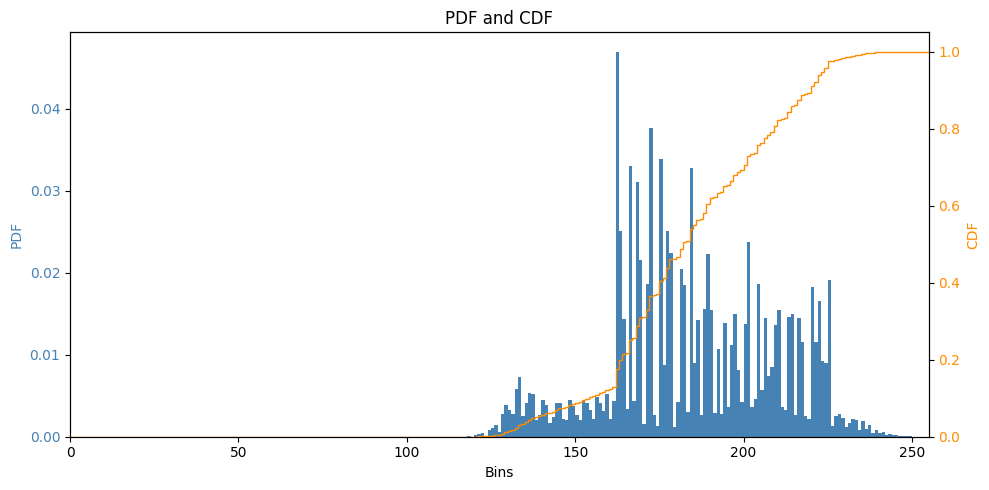
\includegraphics[width=0.9\textwidth]{img/均衡前的直方图.png}
      \caption{均衡前的亮度直方图}
      \label{fig:均衡前的直方图} % 规范命名
    \end{subfigure}
    % \hfill
    \begin{subfigure}{0.45\textwidth}
      \centering
      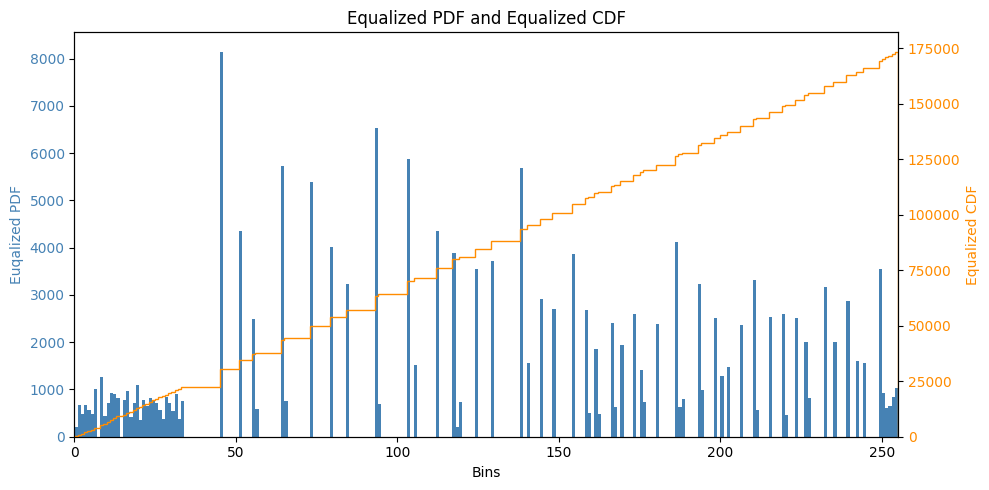
\includegraphics[width=0.9\textwidth]{img/均衡后的直方图.png}
      \caption{均衡后的亮度直方图}
      \label{fig:均衡后的直方图} % 规范命名
    \end{subfigure}
    \caption{直方图均衡前后的亮度直方图和CDF}
    \label{fig:均衡} % 主图标签保持原样
\end{figure}

直方图均衡前后的 I 分量分别如图\ref{fig:original_I}
和图\ref{fig:equalized_I}所示
对比观察图\ref{fig:original_I}和图\ref{fig:equalized_I},
发现均衡后的 I 分量对比度增大,
阴影和高光相较于均衡前更为明显。
\begin{figure}[htbp]
    \centering
    \begin{subfigure}{0.45\textwidth}
      \centering
      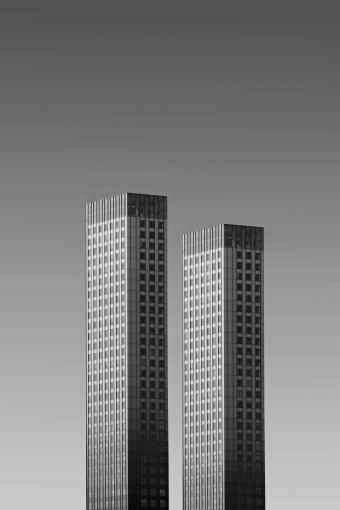
\includegraphics[width=0.8\textwidth]{img/original_I.jpg}
      \caption{均衡前的I分量}
      \label{fig:original_I} % 规范命名
    \end{subfigure}
    % \hfill
    \begin{subfigure}{0.45\textwidth}
      \centering
      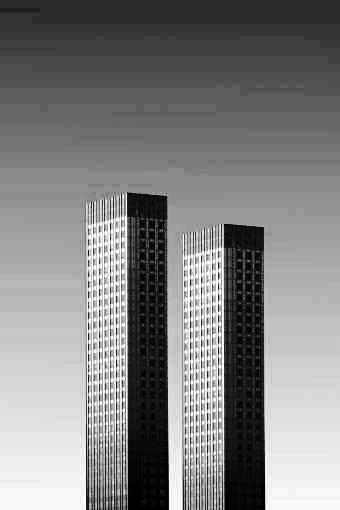
\includegraphics[width=0.8\textwidth]{img/equalized_I.jpg}
      \caption{均衡后的I分量}
      \label{fig:equalized_I} % 规范命名
    \end{subfigure}
    \caption{直方图均衡前后的I分量}
    \label{fig:灰度} % 主图标签保持原样
\end{figure}
\subsection{HSI to RGB}
为了显示直方图均衡后的彩色图像,我们还需要将HSI空间的
图像转换到RHB空间。从HSI空间转换到RGB空间的公式为
式(\ref{eq:hsi2rgb_case1})(\ref{eq:hsi2rgb_case2})
(\ref{eq:hsi2rgb_case3}):

当 \(0 \le H < \tfrac{2\pi}{3}\) 时:
\begin{equation}\label{eq:hsi2rgb_case1}
\begin{aligned}
B &= I\,(1 - S),\\
R &= I\Bigl[1 + \frac{S\,\cos H}{\cos\!\bigl(\tfrac{\pi}{3} - H\bigr)}\Bigr],\\
G &= 3I - (R + B).
\end{aligned}
\end{equation}

当 \(H\) 落在 \(\bigl[\tfrac{2\pi}{3},\,\tfrac{4\pi}{3}\bigr)\) 时,令 \(H' = H - \tfrac{2\pi}{3}\),计算公式为:
\begin{equation}\label{eq:hsi2rgb_case2}
\begin{aligned}
R &= I\,(1 - S),\\
G &= I\Bigl[1 + \frac{S\,\cos H'}{\cos\!\bigl(\tfrac{\pi}{3} - H'\bigr)}\Bigr],\\
B &= 3I - (R + G).
\end{aligned}
\end{equation}

当 \(H\) 落在 \(\bigl[\tfrac{4\pi}{3},\,2\pi\bigr)\) 时,令 \(H'' = H - \tfrac{4\pi}{3}\),计算公式为:
\begin{equation}\label{eq:hsi2rgb_case3}
\begin{aligned}
G &= I\,(1 - S),\\
B &= I\Bigl[1 + \frac{S\,\cos H''}{\cos\!\bigl(\tfrac{\pi}{3} - H''\bigr)}\Bigr],\\
R &= 3I - (G + B).
\end{aligned}
\end{equation}

直方图均衡后HSI图像转换到RGB空间后,如图\ref{fig:equalized_img}
所示,原始图像为图\ref{fig:original}。对比观察图\ref{fig:original}
和图\ref{fig:equalized_img},我们发现原始图像的颜色较淡,图像整体偏亮,
而直方图均衡后的图像,颜色更深,整体亮度适中。尽管亮度直方图均衡
并不会改变色调值和饱和度值,但确实会影响图像的整体颜色。改进方法是,
首先增大图像的饱和度分量,然后再进行亮度直方图均衡化。
\begin{figure}[htbp]
    \centering
    \begin{subfigure}{0.45\textwidth}
      \centering
      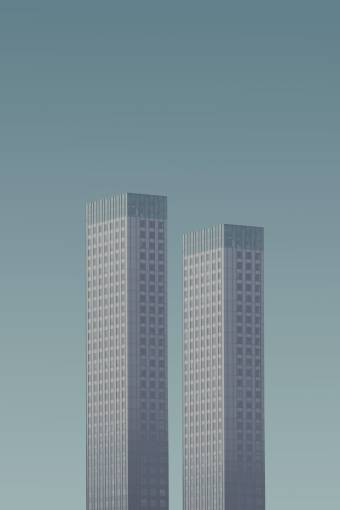
\includegraphics[width=0.8\textwidth]{img/original.jpg}
      \caption{原始图像}
      \label{fig:original} % 规范命名
    \end{subfigure}
    % \hfill
    \begin{subfigure}{0.45\textwidth}
      \centering
      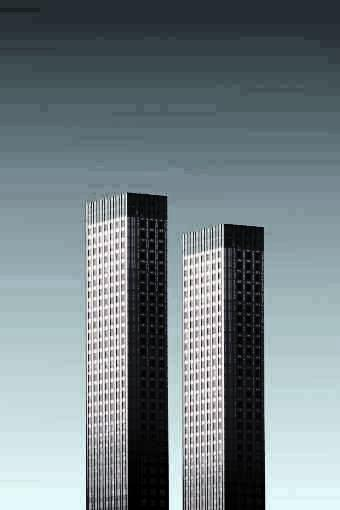
\includegraphics[width=0.8\textwidth]{img/equalized_img.jpg}
      \caption{均衡后的彩色图像}
      \label{fig:equalized_img} % 规范命名
    \end{subfigure}
    \caption{直方图均衡前后的彩色图像}
    \label{fig:前后} % 主图标签保持原样
\end{figure}
\section{问题二}
绿幕抠图系统由两个部分组成,前景图像和背景图像,
前景图像中必须有一个物体放置在绿色的背景之上,
背景图像则可以任意选择。前景图像和背景图像大小必须
相同,抠像系统的输出也与前景和背景大小相同。
在抠图的过程中,我们创建了一个新的图像(输出)。输出
图像的像素依据下面的过程获得:
\begin{enumerate} 
    \item 对前景图像中的每个像素,提取其绿色通道的灰度值; 
    \item 若该灰度值大于设定阈值(如220),则将输出图像中对应位置的像素替换为背景图像中相同位置的像素; 
    \item 否则,保留前景图像中对应位置的像素至输出图像。 
\end{enumerate}
算法流程如算法~\ref{alg:green-screen} 所示。

\begin{algorithm}[H]
    \caption{绿幕抠像算法}
    \label{alg:green-screen}
    \KwIn{前景图像 $F$,背景图像 $B$,阈值 $T$}
    \KwOut{合成图像 $O$}
    \ForEach{像素位置 $(x, y)$}{
      $g \leftarrow F(x, y).\text{G}$ \tcp*{获取绿色通道}
      \eIf{$g > T$}{
        $O(x, y) \leftarrow B(x, y)$ \tcp*{替换为背景像素}
      }{
        $O(x, y) \leftarrow F(x, y)$ \tcp*{保留前景像素}
      }
    }
\end{algorithm}
    
前景,背景和输出图像分别如图\ref{fig:fg},图\ref{fig:bg},图\ref{fig:output}所示:
\begin{figure}[htbp]
    \centering
    \begin{subfigure}{0.33\textwidth}
      \centering
      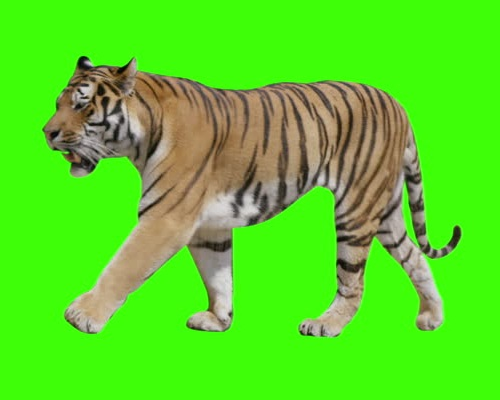
\includegraphics[width=0.8\textwidth]{img/fg.png}
      \caption{前景}
      \label{fig:fg} % 规范命名
    \end{subfigure}
    % \hfill
    \begin{subfigure}{0.33\textwidth}
      \centering
      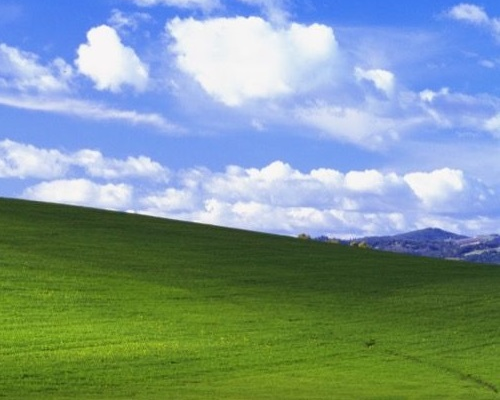
\includegraphics[width=0.8\textwidth]{img/bg.png}
      \caption{背景}
      \label{fig:bg} % 规范命名
    \end{subfigure}
    \begin{subfigure}{0.33\textwidth}
        \centering
        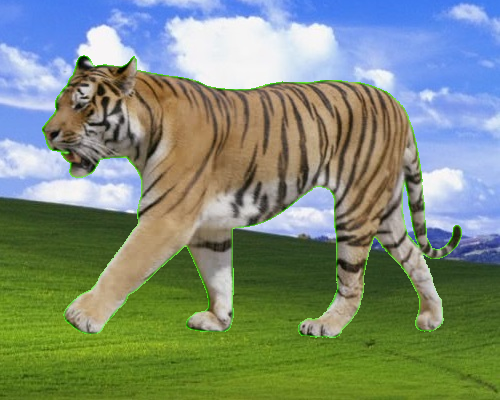
\includegraphics[width=0.8\textwidth]{img/output_img.png}
        \caption{输出图像(T=220)}
        \label{fig:output} % 规范命名
    \end{subfigure}
    \caption{抠像系统的前景、背景和输出}
    \label{fig:前后} % 主图标签保持原样
\end{figure}
观察输出图像,发现抠出的图像存在绿色边框,增大绿色通道的阈值,
边框变厚,如图\ref{fig:outBig},减小绿色通道的阈值,绿色边框变细,但抠出的物体会有像素缺失,如图\ref{fig:outSmall},不能完美的抠出前景中的物体是该抠像算法的局限性。
\begin{figure}[htbp]
    \centering
    \begin{subfigure}{0.45\textwidth}
      \centering
      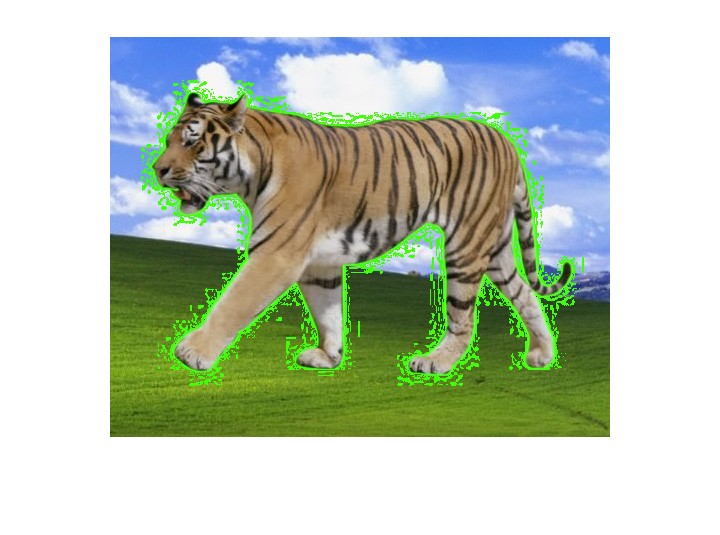
\includegraphics[width=0.9\textwidth]{img/outBig.jpg}
      \caption{阈值T=255}
      \label{fig:outBig} % 规范命名
    \end{subfigure}
    % \hfill
    \begin{subfigure}{0.45\textwidth}
      \centering
      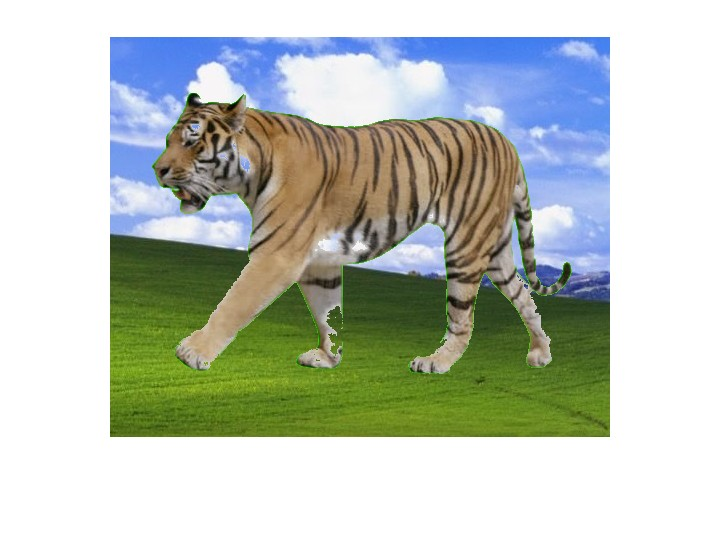
\includegraphics[width=0.9\textwidth]{img/outSmall.jpg}
      \caption{阈值T=200}
      \label{fig:outSmall} % 规范命名
    \end{subfigure}
    \caption{更改阈值后的输出}
    \label{fig:前后} % 主图标签保持原样
\end{figure}
\end{document}